\chapter{\cybersecurityname}
\label{slr_ciber}
Esta sección describe la metodología aplicada en la literatura científica sobre ciberseguridad en la era post-cuántica. Los resultados se presentan junto con un análisis detallado de los hallazgos encontrados.

\section {Metodología}
\label{metodologia}

Para garantizar la validez, transparencia y trazabilidad del proceso, esta revisión adopta un enfoque metodológico basado en el protocolo PICOC. Esta herramienta permite la formulación precisa de preguntas de investigación, la delimitación del alcance temático y la creación de consultas de búsqueda~\cite{CarreraRivera2022}.

\begin{table}[H]
\centering
\caption[Protocolo PICOC - Ciberseguridad post cuántica]{%
    \vspace{4pt}
    \fontsize{12}{11}\selectfont \\
    Protocolo PICOC - Ciberseguridad post cuántica \\[2pt] % Tu subtítulo
}
\label{tab:protocolo_picoc}
\begin{tabular}{@{} l p{10cm} @{}} % Changed L to p
\hline\hline
\textbf{Elemento} & \textbf{Descripción} \\
\hline
Población & Sistemas de información, infraestructuras de red críticas, redes de comunicación, arquitecturas de red seguras y sistemas computacionales expuestos a ciberamenazas post-cuánticas. \\
\hline
Intervención & Adaptación de arquitecturas de red frente a amenazas cuánticas, adopción de tecnologías de ciberseguridad post-cuántica, integración de criptografía post-cuántica e infraestructuras de comunicaciones. \\
\hline
Comparación & Ciberseguridad tradicional, arquitecturas de redes convencionales, y sistemas no preparados para amenazas cuánticas. \\
\hline
Resultados & Mejora de la seguridad en entornos críticos, resiliencia frente a amenazas cuánticas, detección de vulnerabilidades y planificación para una transición tecnológica segura. \\
\hline
Contexto & Transición hacia la era post-cuántica, avance disruptivo de la computación cuántica y creciente necesidad de adaptación de las redes, sistemas digitales e infraestructuras críticas ante futuras amenazas. \\
\hline\hline
\end{tabular}
\end{table}

Tras una cuidadosa evaluación, se formularon las siguientes preguntas de investigación en base a los criterios PICOC establecidos.

\begin{itemize}
    \item Q1: ¿Qué enfoques tecnológicos están siendo propuestos para garantizar la ciberseguridad en un contexto post-cuántico?
    \item Q2: ¿Cómo afecta la computación cuántica a los sistemas de ciberseguridad actuales?
    \item Q3: ¿Qué mecanismos de seguridad habilitan las redes cuánticas para garantizar la confidencialidad e integridad de las comunicaciones en la era post-cuántica?
    \item Q4: ¿Cuáles son los principales desafíos tecnológicos que limitan la evolución de las infraestructuras de seguridad cuántica y qué avances son necesarios para su adopción en sistemas críticos?
\end{itemize}

Para definir la cadena de búsqueda y facilitar la identificación de estudios relevantes, se emplearon las siguientes palabras claves y sinónimos. 

\begin{table}[H]
\centering
\caption[Palabras clave - SLR Ciberseguridad post cuántica]{
    \vspace{4pt}
    \fontsize{12}{11}\selectfont \\
    Palabras clave - SLR Ciberseguridad post cuántica \\[2pt]
}
\label{tab:keywords_slr} % Etiqueta para referenciar esta tabla
\begin{tabular}{@{} l p{6cm} @{}} % Usamos 'l' para Keyword y 'p{6cm}' para Sinónimos con ancho fijo
\hline\hline
\textbf{Palabras clave} & \textbf{Sinónimos} \\
\hline
post-quantum cybersecurity & quantum-safe cybersecurity \\
\hline
quantum cybersecurity & quantum cyber, quantum-enhanced cybersecurity \\
\hline
quantum threat & - \\
\hline
post-quantum security & quantum security \\
\hline
quantum-secured networks & quantum-safe protocols, post-quantum secure protocols \\
\hline\hline
\end{tabular}
\end{table}

Como parte del protocolo metodológico, se diseñó una cadena de búsqueda usando las keywords definidas con el objetivo de identificar y recopilar literatura relevante para esta investigación.

\begin{figure}[H]
\label{searchString}
\centering
\begin{minipage}{0.8\textwidth} % Puedes ajustar el ancho si es necesario
    \centering
    {\fontsize{12}{11}\selectfont % Mantiene el formato del título/subtítulo
     \textbf{Bloque de código 3} \\
     Cadena de Búsqueda - SLR Ciberseguridad post cuántica \\
    }
    \begin{minted}[
        linenos=false, % Sin números de línea
        frame=single, % Con marco
        framesep=2mm, % Separación del marco
        bgcolor=lightgray!20, % Fondo gris claro (ajusta si usas \definecolor{lightgray})
        fontfamily=tt, % Fuente monoespaciada (similar a Courier New)
        fontsize=\small, % Tamaño de fuente pequeño
        obeytabs=true, % Respetar tabulaciones
        tabsize=4, % Tamaño de tabulación
    ]{python}
TITLE-ABS-KEY(
("post-quantum cybersecurity" OR "quantum-safe
cybersecurity") OR
("quantum cybersecurity" OR "quantum cyber" OR "quantum-
enhanced cybersecurity") OR
("post-quantum security" OR "quantum security") OR
("quantum threat") OR
("quantum-secured networks" OR "quantum-safe protocols" OR
"post-quantum secure protocols")
)
AND PUBYEAR > 2020 AND PUBYEAR < 2025
AND (LIMIT-TO (SRCTYPE, "p") OR LIMIT-TO (SRCTYPE, "p"))
AND (LIMIT-TO (SUBJAREA, "COMP") OR LIMIT-TO (SUBJAREA, "ENGI"))
AND (LIMIT-TO (DOCTYPE, "ar") OR LIMIT-TO (DOCTYPE, "cp"))
AND (LIMIT-TO (LANGUAGE, "English"))
    \end{minted}
\end{minipage}
% No hay caption ni label para el bloque de código como una figura normal según tu imagen,
% pero podrías añadirlo si tu plantilla lo espera.
\end{figure}

Adicional a la cadena de búsqueda empleada, se aplicaron filtros para
delimitar los resultados. Se restringió la búsqueda a: 
\begin{itemize}
    \item \textbf{Año de publicación}: 2020-2025
    \item \textbf{Idioma}: Inglés
    \item \textbf{Tipo de publicación}: artículos de revista, actas de congreso y \emph{pre-prints}
    \item \textbf{Área temática}: Ingeniería y Telecomunicaciones
\end{itemize}

Los estudios recopilados, fueron sometidos a filtros de calidad basados en criterios de inclusión y exclusión. Se realizó una selección exhaustiva de artículos no relacionados con nuestro objeto de estudio.

\begin{table}[H]
\centering
\caption[Criterios - Ciberseguridad post cuántica]{
    \vspace{4pt}
    \fontsize{12}{11}\selectfont \\
    Criterios - Ciberseguridad post cuántica \\[2pt]
}
\label{criterios}
\begin{tabular}{@{} p{5.45cm} p{7.973cm} @{}} % Dos columnas de párrafo, ajusta el ancho si es necesario
\hline\hline
\textbf{Inclusión} & \textbf{Exclusión} \\
\hline
\textbf{IC1:} El estudio se centra específicamente en ciberseguridad en entornos post-cuánticos, incluyendo aspectos como redes cuánticas, protocolos quantum-safe, infraestructuras post-cuánticas o criptografía.\par\vspace{8pt}

\textbf{IC2:} El documento analiza o modela amenazas específicas derivadas de la computación cuántica contra sistemas tradicionales de ciberseguridad.\par\vspace{8pt}

\textbf{IC3:} El artículo propone, analiza o evalúa arquitecturas, infraestructuras o estrategias de seguridad en entornos de redes cuánticas.\par\vspace{8pt}

\textbf{IC4:} Se incluyen estudios que aborden desafíos y estrategias de migración, interoperabilidad híbrida o sustitución de algoritmos clásicos en sistemas existentes.

& \textbf{EC1:} Se excluyen estudios centrados exclusivamente en aspectos computacionales, físicos o teóricos de la computación cuántica sin vínculo con la seguridad.\par\vspace{8pt}

\textbf{EC2:} Se excluyen trabajos sobre ciberseguridad tradicional que no contemplen explícitamente el impacto de la computación cuántica, la necesidad de transición post-cuántica o la integración de mecanismo.\par\vspace{8pt}

\textbf{EC3:} Se excluyen estudios de criptografía post-cuántica que no discutan su aplicación práctica en arquitecturas seguras, infraestructuras o redes dentro de la ciberseguridad.\par\vspace{8pt}

\textbf{EC4:} Se excluyen estudios sobre redes cuánticas que se enfoquen exclusivamente en diseño físico, transmisión óptica o aspectos experimentales sin tratar temas de integridad, confidencialidad o autenticación.\par\vspace{8pt}

\textbf{EC5:} Se excluyen trabajos que no presentan una contribución significativa al campo de la ciberseguridad post-cuántica y muestran baja relevancia académica.
\\
\hline\hline
\end{tabular}
\end{table}

\section{Modelo PRISMA}

Para estructurar y documentar de forma rigurosa el proceso de selección de estudios, se ha seguido la metodología PRISMA (Preferred Reporting Items for Systematic Reviews and Meta-Analyses)~\cite{Page2021}. Este modelo proporciona una guía estandarizada que permite garantizar la transparencia, la reproducibilidad y la trazabilidad en revisiones sistemáticas, desde la fase de identificación de fuentes hasta la inclusión final de los estudios relevantes.

\begin{figure}[H]
\centering
\caption[Modelo PRISMA - Ciberseguridad Post Cuántica]{%
    \vspace{4pt}
    \fontsize{12}{11}\selectfont \\
    Modelo PRISMA - Ciberseguridad Post Cuántica \\
}
\footnotesize Fuente: Elaboración propia
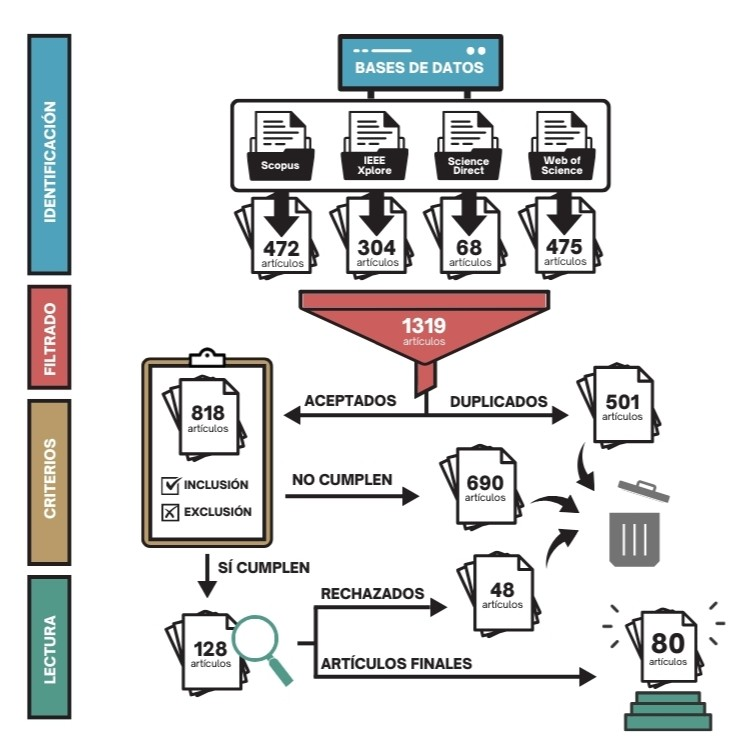
\includegraphics[width=0.93\textwidth]{pictures/Modelo_PRISMA_SLRCiber.jpg}
\label{fig:modelo_prisma}
\end{figure}

Inicialmente, se recopilaron 1319 artículos de las bases de datos. Tras una fase de filtrado, se eliminaron 501 duplicados, resultando en 818 artículos únicos para una revisión detallada. De estos, se aceptaron 128 artículos que cumplieron con los criterios de inclusión/exclusión, mientras que 690 fueron rechazados. Finalmente, los 128 artículos aceptados fueron sometidos a una lectura completa y una evaluación de calidad, culminando con la selección de 80 artículos finales que constituyen la base de esta SLR.

\section{Análisis de Resultados}

El mundo cuántico es un campo de estudio que se encuentra en fases muy preliminares de desarrollo y adopción. Por esta razón, la revisión sistemática se ha centrado exclusivamente en artículos publicados entre los años 2020 a 2025.
Esta limitación temporal es fundamental para analizar el estado actual de la investigación, artículos anteriores a este periodo podrían no ser relevantes para comprender las tendencias y desafíos emergentes.

Con ese mismo objetivo de capturar las contribuciones más recientes y significativas, se decido incluir \emph{pre-prints} en la revisión. Estos documentos, aunque no han pasado por un proceso formal de revisión por pares, a menudo contienen información crucial en campos tan dinámicos como la cuántica. 

A continuación, se presenta una gráfica que muestra la distribución temporal junto a na clasificación detallada de los tipos de artículos considerados en esta revisión sistemática.

\begin{figure}[H]
\centering
\caption[Año de publicación y tipo de artículo - Ciberseguridad Post Cuántica]{
    \vspace{4pt}
    \fontsize{12}{11}\selectfont \\
    Año y Tipo de publicación - Ciberseguridad Post Cuántica \\
}
\footnotesize Fuente: Elaboración propia
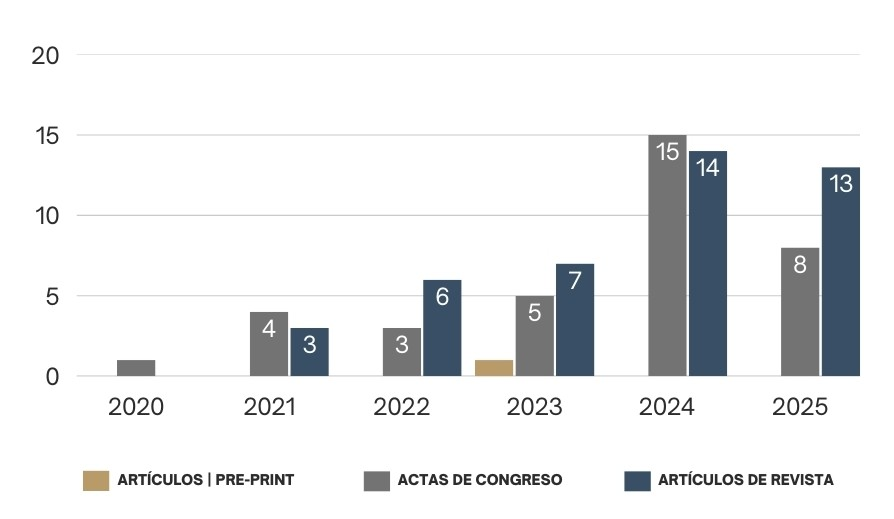
\includegraphics[width=0.95\textwidth]{pictures/Años_Tipos_SLRCiber.jpg}
\label{fig:año_tipo}
\end{figure}

Continuando con el análisis, los artículos fueron agrupados en categorías que reflejan las áreas más relevantes y recurrentes dentro del campo de la ciberseguridad en la era post-cuántica.

Las cinco temáticas identificadas tras analizar la totalidad de los artículos recopilados son las siguientes:
\begin{itemize}
    \item \textbf{Criptografía Post-Cuántica (PQC)}: Engloba propuestas y evaluaciones de algoritmos resistentes a ataques de computadoras cuánticas, con énfasis en estándares emergentes y esquemas criptográficos alternativos.
    \item \textbf{Seguridad en Redes y Comunicaciones}: Incluye investigaciones centradas en proteger la integridad, confidencialidad y disponibilidad de sistemas de comunicación frente a amenazas cuánticas, especialmente en contextos como IoT, 5G o redes definidas por software.
    \item \textbf{Marcos y Soluciones Integradas de Seguridad Cuántica}: Agrupa propuestas de arquitecturas, infraestructuras o sistemas completos que incorporan protección cuántica en distintos niveles del ecosistema tecnológico.
    \item \textbf{Distribución Cuántica de Claves (QKD)}: Reúne estudios centrados en el uso de principios de la mecánica cuántica para el intercambio seguro de claves criptográficas, así como sus aplicaciones y limitaciones prácticas.
    \item \textbf{Ataques y Amenazas Cuánticas}: Incluye trabajos que analizan posibles vectores de ataque derivados del uso de tecnologías cuánticas, así como la evaluación del impacto potencial sobre los sistemas tradicionales de seguridad.
\end{itemize}

\begin{figure}[H]
\centering
\caption[Artículos por campo de estudio - Ciberseguridad Post Cuántica]{
    \vspace{4pt}
    \fontsize{12}{11}\selectfont \\
    Artículos por campo de estudio - Ciberseguridad Post Cuántica \\
}
\footnotesize Fuente: Elaboración propia
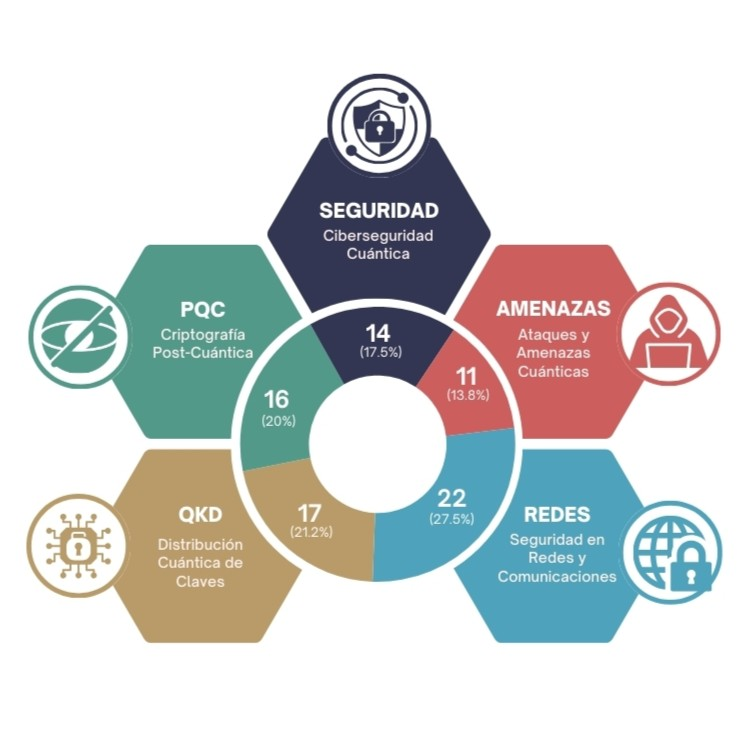
\includegraphics[width=0.90\textwidth]{pictures/Campos_Estudio_SLRCiber.jpg}
\label{fig:campo_estudio_SLRCiber}
\end{figure}

Como extensión del análisis temático, se llevó a cabo un estudio de la frecuencia de palabras clave identificando así los conceptos más recurrentes en la literatura recopilada y verificar su alineación con las categorías definidas previamente.

\begin{figure}[H]
\centering
\caption[Frecuencia de palabras clave - Ciberseguridad Post Cuántica]{
    \vspace{4pt}
    \fontsize{12}{11}\selectfont \\
    Frecuencia de palabras clave - Ciberseguridad Post Cuántica \\
}
\footnotesize Fuente: Elaboración propia
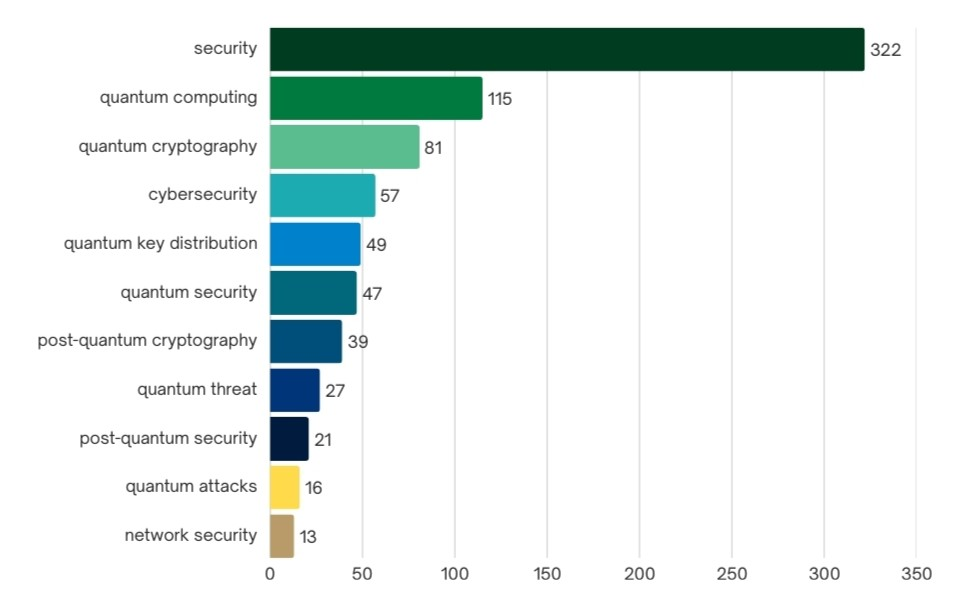
\includegraphics[width=0.90\textwidth]{pictures/Keywords_SLRCiber.jpg}
\label{fig:keywords}
\end{figure}

De forma complementaria se presenta un estudio sobre el número de citaciones con el que se pretende identificar los trabajos de mayor impacto en la comunidad científica.
En primer lugar, se presenta una lista con los diez artículos más citados. La importancia de estas publicaciones no solo radica en su contenido técnico, sino también en su capacidad de influir en líneas de investigación futuras y orientar estándares emergentes.
Además de este análisis individual, se ha realizado un estudio generalizado de citaciones por campo temático, utilizando las categorías definidas previamente. Este enfoque permite observar qué áreas están generando mayor atención y reconocimiento en la comunidad investigadora, lo que puede interpretarse como una señal indirecta de madurez o urgencia científica.

\begin{longtable}{@{} p{10.5cm} c @{}}
\caption[Artículos más citados - Ciberseguridad Post Cuántica]{
    \vspace{4pt}
    \fontsize{12}{11}\selectfont \\
    Artículos más citados - Ciberseguridad Post Cuántica \\[2pt]
}
\label{tab:articulos_mas_citados}\\
\hline 
\noalign{\vskip 2pt} 
\hline
\textbf{Artículo} & \textbf{Citas} \\
\hline
\endfirsthead

\hline 
\endhead

\hline
\endfoot

\hline 
\noalign{\vskip 2pt} 
\hline
\endlastfoot

Quantum2FA: Efficient Quantum-Resistant Two-Factor Authentication Schemefor Mobile Devices (2023)~\cite{Wang2023} & 162 \\
\hline % Single line for each row
A Review of Quantum Cybersecurity: Threats, Risks and Opportunities (2022)~\cite{HossainFaruk2022} & 123 \\
\hline % Single line for each row
Quantum Cryptography in 5G Networks: A Comprehensive Overview (2024)~\cite{Mehic2024} & 84 \\
\hline % Single line for each row
KaLi: A Crystal for Post-Quantum Security Using Kyber and Dilithium (2023)~\cite{Aikata2023} & 83 \\
\hline % Single line for each row
Quantum-Inspired Machine Learning for 6G: Fundamentals, Security,Resource Allocations, Challenges, and Future Research Directions (2022)~\cite{Duong2022} & 78 \\
\hline % Single line for each row
The Future of Cybersecurity in the Age of Quantum Computers (2022)~\cite{Raheman2022} & 69 \\
\hline % Single Line for each row
Quantum Computing For Cryptographic Security With Artificial Intelligence (2024)~\cite{Vadisetty2024} & 67 \\
\hline % Single line for each row
Lattice-based cryptosystems for the security of resource-constrained IoTdevices in post-quantum world: a survey (2022)~\cite{Seyhan2022} & 64 \\
\hline % Single line for each row
Network Coding-Based Post-Quantum Cryptography (2021)~\cite{Cohen2021} & 63 \\
\hline % Single line for each row
On The Use of Quantum Communications for Securing IoT Devices in the 6G era (2021)~\cite{AlMohammed2021} & 53 \\
\end{longtable}


\begin{figure}[H]
\centering
\caption[Citaciones por campo de estudio - Ciberseguridad Post Cuántica]{
    \vspace{4pt}
    \fontsize{12}{11}\selectfont \\
    Citaciones por campo de estudio - Ciberseguridad Post Cuántica \\
}
\footnotesize Fuente: Elaboración propia
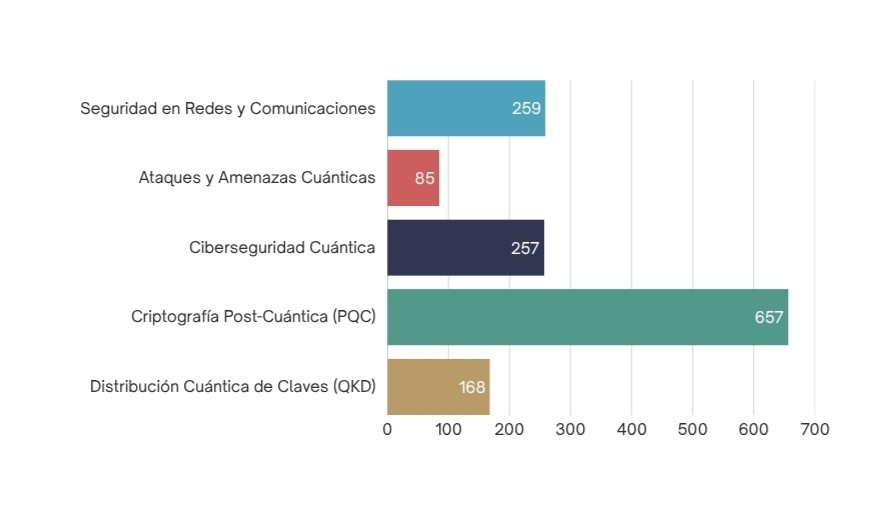
\includegraphics[width=0.95\textwidth]{pictures/Citas__SLRCiber.jpg}
\label{fig:Citas__SLRCiber}
\end{figure}

\section{Análisis Preguntas de Investigación}

Esta sección ofrece una respuesta estructurada y detallada a las preguntas de investigación formuladas al inicio de esta revisión sistemática.

\vspace{1em} \textbf {Q1: ¿Qué enfoques tecnológicos están siendo propuestos para garantizar la ciberseguridad en un contexto post-cuántico?}

Se busca identificar soluciones tecnológicas en desarrollo que guiarán la transición hacia nuevas arquitecturas de seguridad. Estas soluciones deben proteger las infraestructuras digitales y garantizar resiliencia frente a las amenazas que la computación cuántica podría introducir en la próxima era tecnológica.

\begin{longtable}{@{} p{4.5cm} p{6.5cm} c c @{}}
\caption[Q1 - Ciberseguridad Post Cuántica]{
  \vspace{4pt}
  \fontsize{12}{11}\selectfont \\
   Q1 - Ciberseguridad Post Cuántica \\[2pt]
}
\label{tab:q1_slr}\\
\hline 
\noalign{\vskip 2pt} 
\hline
\textbf{Artículo} & \textbf{Descripción} & \textbf{Año} & \textbf{Citas} \\
\hline 
\endfirsthead
\hline
\endhead
\hline
\endfoot
\hline 
\noalign{\vskip 2pt} 
\hline
\endlastfoot

Post-Quantum MACsec in Ethernet Networks~\cite{Cho2021} & Propone un protocolo de establecimiento de claves post-cuántico autenticado para MACsec, asegurando redes Ethernet frente a ataques cuánticos. & 2021 & 12 \\
\hline 
A Review of the Present Cryptographic Arsenal to Deal with Post-Quantum Threats~\cite{YALAMURI2022} & Revisa y categoriza las principales familias de Criptografía Post-Cuántica (PQC) como enfoques fundamentales para mitigar amenazas cuánticas. & 2022 & 47 \\
\hline
Towards Post-Quantum Security for Cyber-Physical Systems: Integrating PQC into Industrial M2M Communication~\cite{Paul2020} & Propone e implementa soluciones híbridas y puramente PQC para integrar criptografía post-cuántica en sistemas ciber-físicos industriales. & 2020 & 22 \\
\hline
LPQAA: a lightweight post-quantum access authentication scheme for satellite network~\cite{Wang2025} & Propone un esquema de autenticación de acceso basado en retículos para redes satelitales, resistente a ataques cuánticos. & 2025 & 0 \\
\hline
A comprehensive and realistic performance evaluation of post-quantum security for consumer IoT devices~\cite{HANNA2025} & Investiga y el rendimiento de algoritmos post-cuánticos en la seguridad TLS para dispositivos IoT de consumo. & 2025 & 0 \\
\hline
A Framework for Migrating to Post-Quantum Cryptography: Security Dependency Analysis and Case Studies~\cite{Hasan2024} & Presenta un marco integral y sistemático para ayudar a las organizaciones en el proceso de migrar sus activos criptográficos a soluciones cuántico-resistentes. & 2024 & 39 \\
\hline
Quantum Computing and Cryptography in Cybersecurity: A Disruptive Synergy~\cite{Maqousi2025} & Examina las vulnerabilidades de la criptografía actual ante la computación cuántica, investigando nuevos métodos resistentes a la cuántica y proponiendo enfoques híbridos para la transición. & 2025 & 0 \\
\hline
Securing the Internet of Things with Ascon-Sign~\cite{MAGYARI2024} & Presenta método para mejorar la seguridad en dispositivos del Internet de las Cosas (IoT). & 2024 & 2 \\
\hline
KaLi: A Crystal for Post-Quantum Security Using Kyber and Dilithium~\cite{Aikata2023} & Presenta una metodología de diseño y una arquitectura unificada para la implementación eficiente de los esquemas criptográficos post-cuánticos NIST CRYSTALS-Dilithium y CRYSTALS-Kyber. & 2023 & 83 \\
\hline
A Multi-Layered Quantum-Resistant Algorithms Based Approach to Mitigate Emerging Threats in ISP Cybersecurity~\cite{Alagh2024} & Propone una serie de algoritmos criptográficos multicapa cuántico-resistentes para su integración en redes de Proveedores de Servicios de Internet (ISP), fortaleciendo su ciberseguridad. & 2024 & 1 \\
\end{longtable}

\vspace{1em} \textbf {Q2: ¿Cómo afecta la computación cuántica a los sistemas de ciberseguridad actuales?}

La formulación de esta pregunta surge de la necesidad de entender cómo la computación cuántica afecta a la seguridad de los sistemas actuales. Al analizar este tema, se busca comprender el impacto de sus avances, identificar riesgos críticos y determinar qué protocolos o arquitecturas necesitan ser actualizados o reemplazados.

\begin{longtable}{@{} p{4.5cm} p{6.5cm} c c @{}}
\caption[Q2 - Ciberseguridad Post Cuántica]{
   \vspace{4pt}
   \fontsize{12}{11}\selectfont \\
   Q2 - Ciberseguridad Post Cuántica \\[2pt]
}
\label{tab:q2_slr}\\
\hline
\noalign{\vskip 2pt}
\hline 
\textbf{Artículo} & \textbf{Descripción} & \textbf{Año} & \textbf{Citas} \\  
\hline 
\endfirsthead
\hline
\endhead
\hline
\endfoot
\hline
\noalign{\vskip 2pt} 
\hline
\endlastfoot

A Review of Quantum Cybersecurity: Threats, Risks and Opportunities~\cite{HossainFaruk2022} & Revisa las amenazas y riesgos emergentes que la computación cuántica introduce para la ciberseguridad, explorando cómo transforma el panorama actual. & 2022 & 123 \\
\hline
Quantum Attacks on Blockchain and Mitigation Strategies~\cite{RM2025} & Analiza la capacidad de la computación cuántica para romper el cifrado de las tecnologías blockchain, identificando esta como una amenaza inminente para los sistemas descentralizados actuales. & 2025 & 0 \\
\hline
Hacking Cryptographic Protocols with Advanced Variational Quantum Attacks~\cite{Aizpurua2025} & Demuestra cómo algoritmos avanzados de ataque cuántico pueden comprometer eficientemente protocolos criptográficos simétricos, reduciendo significativamente las iteraciones necesarias para encontrar claves. & 2025 & 7 \\
\hline
The Future of Cybersecurity in the Age of Quantum Computers~\cite{Raheman2022} & Aborda el impacto directo y preocupante de la computación cuántica al señalar cómo algoritmos de PQC que se consideraban seguros ya no lo son. & 2022 & 69 \\
\hline
Evaluation framework for quantum security risk assessment: A comprehensive strategy for quantum-safe transition~\cite{BASERI2025} & Explora cómo la computación cuántica representa una amenaza significativa para las medidas de seguridad criptográficas tradicionales, invalidando algoritmos asimétricos y exigiendo una reevaluación urgente del riesgo para la transición. & 2025 & 1 \\
\hline
QIris: Quantum Implementation of Rainbow Table Attacks~\cite{Quan2025} & Explora el uso del Algoritmo de Grover para mejorar drásticamente la eficiencia de los ataques de tabla arcoíris, demostrando cómo la computación cuántica puede acelerar las herramientas de descifrado de contraseñas y afectar la ciberseguridad. & 2025 & 1 \\
\hline
Towards Discovering Quantum-Threats for Applications Using Open-Source Libraries~\cite{Ye2024} & Investiga la exposición de aplicaciones actuales a amenazas cuánticas al identificar el uso de algoritmos criptográficos clásicos vulnerables (RSA, DH, ECC) en bibliotecas de código abierto. & 2024 & 0 \\
\hline
Quantum security of Trojan message attacks on Merkle-Damgård hash construction~\cite{Xu2025} & Analiza cómo los ataques troyano pueden mejorarse significativamente con computadoras cuánticas. & 2025 & 0 \\
\hline
Analyzing the Data of Software Security Life-Span: Quantum Computing Era~\cite{Alyami2022} & Discute cómo la emergencia de la computación cuántica afecta la vida útil y resiliencia de las soluciones de seguridad de software actuales, señalando la necesidad de reevaluar y adaptar las metodologías existentes. & 2022 & 18 \\
\hline
NISQ Quantum Computing: A Security-Centric Tutorial and Survey~\cite{Chen2024} & El artículo identifica y clasifica vulnerabilidades en sistemas de computación cuántica para mejorar su seguridad y mitigar amenazas. & 2024 & 12 \\
\end{longtable}

\vspace{1em} \textbf {Q3: ¿Qué mecanismos de seguridad habilitan las redes cuánticas para garantizar la confidencialidad e integridad de las comunicaciones en la era post-cuántica?}

Se busca analizar cómo las redes cuánticas pueden salvaguardar la información frente amenazas tanto clásicas como cuánticas. Esta cuestión nos permite explorar mecanismos de protección específicos incluyendo protocolos, medidas de cifrado, evaluar su viabilidad en entornos reales e industriales, incluso determinar las limitaciones técnicas que podrían afectar su implementación a gran escala.


\begin{longtable}{@{} p{4.5cm} p{6.5cm} c c @{}}
\caption[Q3 - Ciberseguridad Post Cuántica]{
   \vspace{4pt}
   \fontsize{12}{11}\selectfont \\
   Q3 - Ciberseguridad Post Cuántica \\[2pt]
}
\label{tab:q3_slr}\\ 
\hline
\noalign{\vskip 2pt}
\hline
\textbf{Artículo} & \textbf{Descripción} & \textbf{Año} & \textbf{Citas} \\
\hline
\endfirsthead
\hline
\endhead
\hline
\endfoot
\hline
\noalign{\vskip 2pt} 
\hline
\endlastfoot

Combined Quantum and Post-Quantum Security for Earth-Satellite Channels~\cite{Rani2025} & Demuestra un sistema prototipo de distribución de clave cuántica (QKD) integrado con criptografía post-cuántica para asegurar comunicaciones en canales satelitales, garantizando confidencialidad e integridad. & 2025 & 2 \\
\hline
Navigating quantum security risks in networked environments: A comprehensive study of quantum-safe network protocols~\cite{BASERI2024} & Analiza las vulnerabilidades de los protocolos de red actuales frente a ataques cuánticos y evalúa la efectividad de las soluciones criptográficas post-cuánticas para la seguridad en entornos de red. & 2024 & 39 \\
\hline
Quantum Key Distribution-Based Security Framework for Wireless Sensor Networks: Enhancing Resilience Against Classical and Quantum Cyber Threats~\cite{Senthilkumar2024} & Propone un marco de seguridad basado en la Distribución de Clave Cuántica (QKD) para redes de sensores inalámbricos, buscando proteger los datos y garantizar su confidencialidad frente a amenazas cuánticas. & 2024 & 0 \\
\hline
Space enabled secure quantum communication~\cite{Lazzaro2024} & Destaca las ventajas del espacio como medio de comunicación, permitiendo una seguridad inquebrantable para redes de información cuántica. & 2024 & 0 \\
\hline
Quantum Cryptography in 5G Networks: A Comprehensive Overview~\cite{Mehic2024} & Ofrece una visión general de cómo las técnicas de criptografía cuántica se utilizan para establecer claves criptográficas resistentes a ataques cuánticos en entornos de redes 5G, crucial para la seguridad de las comunicaciones. & 2024 & 84 \\
\hline
Exploring the fusion of lattice-based quantum key distribution for secure Internet of Things communication~\cite{Biswas2024} & Propone una fusión de la criptografía basada en retículos con protocolos de Distribución de Clave Cuántica (QKD) para establecer canales de comunicación seguros y robustos en ecosistemas IoT. & 2024 & 8 \\
\hline
On The Use of Quantum Communications for Securing IoT Devices in the 6GEra~\cite{AlMohammed2021} & Propone el uso de QKD para cifrar datos en dispositivos IoT, ofreciendo un método de seguridad robusto frente a ataques cuánticos. & 2021 & 53 \\
\hline
Cross-layering consideration for network and quantum resources-aware quantum-secured networking~\cite{LEE2025} & Investiga algoritmos para redes seguras cuánticamente, que combinan capas de red de usuario con redes de distribución de clave cuántica (QKDN) para una gestión eficiente. & 2025 & 1 \\
\hline
Quantum2FA: Efficient Quantum-Resistant Two-Factor Authentication Schemefor Mobile Devices~\cite{Wang2023} & Propone un esquema de autenticación de dos factores (2FA) resistente a la cuántica basado en tarjetas inteligentes, abordando la necesidad de seguridad y eficiencia en dispositivos móviles frente a ataques cuánticos. & 2023 & 162 \\
\end{longtable}

\vspace{1em} \textbf {Q4: ¿Cuáles son los principales desafíos tecnológicos que limitan la evolución de las infraestructuras de seguridad cuántica y qué avances son necesarios para su adopción en sistemas críticos?}

Esta pregunta esta centrada en los desafíos que dificultan la implementación efectiva de tecnologías cuánticas en el ámbito de la ciberseguridad. Se analizan aspectos como la escalabilidad, la interoperabilidad, los costos, la estandarización y las limitaciones técnicas para integrar redes e infraestructuras cuánticas en los entornos existentes.

\begin{longtable}{@{}  p{4.5cm} p{6.5cm} c c @{}}
\caption[Q4 - Ciberseguridad Post Cuántica]{
   \vspace{4pt}
   \fontsize{12}{11}\selectfont \\
   Q4 - Ciberseguridad Post Cuántica \\[2pt]
}
\label{tab:q4_slr}\\ 
\hline 
\noalign{\vskip 2pt} 
\hline 
\textbf{Artículo} & \textbf{Descripción} & \textbf{Año} & \textbf{Citas} \\
\hline 
\endfirsthead
\hline 
\endhead
\hline
\endfoot
\hline
\noalign{\vskip 2pt}
\hline
\endlastfoot

Trojan Taxonomy in Quantum Computing~\cite{Das2024} & Desarrolla una taxonomía estructurada de troyanos para sistemas de información cuántica, abordando los desafíos de vulnerabilidades específicas en el hardware y software cuántico que limitan su evolución segura. & 2024 & 3 \\
\hline
Quantum-driven zero trust architecture with dynamic anomaly detection in 7G technology: A neural network approach~\cite{Ahmed2025} & Propone una arquitectura Zero Trust mejorada con Redes Neuronales Cuánticas, reconociendo que la adopción de la ciberseguridad cuántica está limitada por la escalabilidad, la eficiencia en la codificación de datos y los altos costos computacionales. & 2025 & 0 \\
\hline
Quantum Blockchain for Internet of Things: A systematic review, proposed solutions and challenges~\cite{Chawla2025} & Revisa las vulnerabilidades de los sistemas blockchain actuales frente a ataques cuánticos y enfatiza en la importancia de integrar la tecnología de Blockchain Cuántico en IoT. & 2025 & 0 \\
\hline
The complex path to quantum resistance~\cite{Mashatan2021} & Ofrece recomendaciones y una hoja de ruta para la transición hacia una seguridad resistente a la cuántica, abordando los desafíos de la implementación holística en organizaciones. & 2021 & 12 \\
\hline
Overview of Security Approaches for Quantum Computing in the Current Era~\cite{Hansora2025} & Aborda una visión general de las amenazas de ciberseguridad que introduce la computación cuántica y las diferentes preocupaciones de seguridad en la era actual, destacando los desafíos inherentes a la tecnología. & 2025 & 0 \\
\hline
European Quantum ecOsystems - Preparing the Industry for the Quantum Security and Communications Revolution~\cite{Farrugia2024} & Enfatiza la urgencia de preparar a la industria para la revolución cuántica, destacando la necesidad de soluciones (QKD y PQC) frente a la amenaza de los ordenadores cuánticos que comprometen la ciberseguridad actual. & 2024 & 1 \\
\hline
Towards a Quantum-Resilient Future: Strategies for Transitioning to Post-Quantum Cryptography~\cite{Aydeger2024} & Propone una estrategia integral para la transición a la criptografía post-cuántica, abordando su desarrollo, herramientas de implementación a gran escala, sistemas híbridos y consideraciones regulatorias. & 2024 & 32 \\
\hline
Enhancing IoT Security: Quantum-Level Resilience against Threats~\cite{Alhakami2024} & Examina la necesidad de seguridad cuántica en IoT, investigando la integración de enfoques cuánticos y protocolos criptográficos para proteger datos y la integridad de sistemas IoT. & 2024 & 10 \\
\hline
PQC Secure: Strategies for Defending Against Quantum Threats~\cite{Jenefa2023} & Evalúa la eficacia de la PQC como solución a las amenazas cuánticas, analizando métricas de rendimiento y subrayando la importancia de la transición a PQC para la seguridad de la información. & 2023 & 9 \\
\hline
Post-quantum cryptographic assemblages and the governance of the quantum threat~\cite{Csenkey2023} & Explora la gobernanza y las políticas para gestionar la amenaza cuántica, identificando la infraestructura, estandarización y educación como claves en la preparación estatal e industrial. & 2023 & 27 \\
\end{longtable}

\section{Hallazgos y nuevas líneas futuras}

La computación cuántica emergente supone una amenaza por su gran potencial para desafiar los fundamentos de la ciberseguridad actual. Dentro de este contexto, la criptografía, pilar esencial de la seguridad de la información, es el campo más vulnerable ante las capacidades cuánticas. La investigación muestra que algoritmos cuánticos como los de Shor y Grover representan un gran riesgo para métodos criptográficos ampliamente usados como RSA, ECC y las funciones hash. Además, las tecnologías cuánticas tienen el potencial de acelerar ataques conocidos como los de tabla arcoíris o DNS. La preocupación también se extiende a la vida útil de la seguridad del software y a la vulnerabilidad de sistemas y aplicaciones que actualmente emplean criptografía susceptible a estos ataques. Todos estos hallazgos resaltan la importancia de reevaluar los riesgos y comenzar a planear una transición hacia soluciones que puedan resistir los efectos de la computación cuántica.

Frente a esta amenaza, la comunidad investigadora está desarrollando activamente nuevos enfoques. Por un lado, la Criptografía Post-Cuántica (PQC) se presenta como una solución clave. Se están investigando varias familias de PQC, como las basadas en retículos, funciones hash o códigos, con el objetivo de reemplazar las primitivas criptográficas tradicionales e integrar estas técnicas en una variedad de aplicaciones, desde redes Ethernet y sistemas ciberfísicos, hasta redes satelitales y dispositivos IoT. Esto incluye desarrollar esquemas de PQC para crear claves, la autenticación y la firma digital, así como el diseño de arquitecturas multicapa que mejoren la ciberseguridad en infraestructuras grandes. La velocidad y eficiencia en la implementación de algoritmos estandarizados, como CRYSTALS-Dilithium y Kyber, muestran que esta área está creciendo rápidamente~\cite{NIST2021Ready}. 

Por otro lado, la Distribución de Clave Cuántica (QKD) va ganando terreno como un método de seguridad basado en las leyes de la física, lo que la hace incondicionalmente segura, algo que la criptografía clásica no puede ofrecer. Se están explorando diversas formas de implementarla en diferentes tipos de redes, incluyendo enlaces Tierra-Satélite, redes 5G y futuras 6G, hasta redes de sensores inalámbricos (WSN) y dispositivos IoT. La QKD da una manera sólida de crear claves secretas que son seguras contra cualquier adversario, incluso aquellos equipados con computadoras cuánticas avanzadas. Una tendencia significativa es combinar QKD con PQC, formando soluciones híbridas que aprovechan la seguridad teórica incondicional de QKD y la flexibilidad de PQC para ofrecer un sistema de comunicaciones más completo y resistente. La gestión eficiente de claves cuánticas y el monitoreo constante de amenazas durante el proceso de distribución son áreas de intensa investigación actual~\cite{Hansora2025}. 

Sin embargo, avanzar hacia una ciberseguridad resistente a la computación cuántica conlleva varios desafíos tecnológicos importantes. La migración en sí misma no es sencilla, demanda una planificación estratégica, el desarrollo de nuevas competencias y marcos metodológicos dentro de las organizaciones. Desde el punto de vista tecnológico, la escalabilidad y la eficiencia de las soluciones cuánticas aún presentan limitaciones significativas.  La industria aún necesita prepararse adecuadamente para comprender y adoptar estas innovaciones con éxito.
